\documentclass{beamer}
\usepackage[utf8]{inputenc}
\usepackage[french]{babel}
\usepackage{graphicx}

% 20 minutes presentation time

\title{Investigation sur les différences dans les interactions
  enseignant-élèves selon le sexe de l’élève dans les classes
  de physique}
\subtitle{Une étude pilote }
\author{Sofia Vallecorsa \& Paul Maley}
\date{29 juin 2017}

\begin{document}

%% Titlepage
\frame{\titlepage}

%% TOC
\begin{frame}
\frametitle{Table de matières}
\tableofcontents
\end{frame}

%% Introduction
\section{Introduction}
\begin{frame}
\frametitle{Introduction}
\begin{itemize}
\item L'inégalité d'emploi entre hommes et femmes dans les métiers STEM est une évidence.
\item Les origines de cet inégalité (sur tout concernant le part joué par la scolarité) sont le sujet de beaucoup d'études.
\item Notre projet propose d'investiguer une seule cause potentielle parmi beaucoup -- l'interaction enter enseignant et élève.
\end{itemize}
\end{frame}

%% Problématique
\section{Problématique}
\begin{frame}
\frametitle{Problématique}
\begin{block}{ }
Y a-t-il une différentiation dans les interactions enseignants-élèves entre les élèves masculins et les élèves féminines dans les écoles secondaires en Suisse Romandes?'
\end{block}
\end{frame}

%% Méthodologie
\section{Méthodologie}
\subsection{Méthodologie standarde}
\begin{frame}
\frametitle{Méthodologie standarde}
\begin{itemize}
\item La méthodologie ``standarde'' pour chercher une telle différence serait d'enregistrer des séance de classe et d'analyser
les interactions selon un cadre théorique. La théorie des actions didactiques conjoints (TADC) semble être un bon choix.
\item Une telle analyse permettrait d'observer des différences mais pour en venir à la raison d'être de ces différences il faudrait articuler ces obsevations avec des entretiens enseignants.
\item Pour comprendre si ces différences sans généralisés ou des cas isolés il en faudra beaucoup de vidéos.
\item Cette approche est limitée par le temps qu'il faut pour analyser des séquences vidéos mais aussi par des questions
légales -- vision des vidéos par autrui.  
\end{itemize}
\end{frame}

\subsection{Notre approche}
\begin{frame}
\frametitle{Notre approche -- le questionnaire}
\begin{itemize}
\item Nous avons imaginé une approche alternative.
\item Utiliser un questionnaire où chaque question propose:
  \begin{itemize}
   \item Une situation et le début d'une transaction didactique en classe
   \item Deux options pour comment poursuivre la transaction 
  \end{itemize}
\item Le questionnaire est presenté aux répondants comme une étude sur
  ``la posture didactique'' de l'enseignant(e).
\item Le répondant est encouragé de visualiser la situation et choisir la
  réponse la plus apte. 
\end{itemize}
\end{frame}

\begin{frame}
\frametitle{Notre approche -- fonctionnement}
\begin{itemize}
\item Le questionnaire existe en deux version: A/B.
\item Dans chaque question le sexe de l'élève est inversé entre les questionnaires.
\item Un intéraction différencié selon le sexe se manifeste dans une différence
dans la proportion de chaque réponse choisit entre les deux questionnaires (A/B). 
  
\end{itemize}
\end{frame}


\begin{frame}
\frametitle{Notre approche -- Un exemple (Version A)}
\begin{block}{Question – Classe 1M}
Vous demandez à la classe la distance approximative entre la lune et la terre (sujet discuté la veille) et plusieurs élèves (Zoe entre eux) lèvent la main. Vous donnez la parole à Zoe mais elle hésite :
\end{block}

\begin{block}{Réponses}
\begin{itemize}
\item Vous attendez quelques secondes pour sa réponse.
\item Vous passez à quelqu’un d’autre (ça doit être une simple restitution).
\end{itemize}
\end{block}

Version B est pareil avec Zoe remplacé par Nathan.
\end{frame}

\begin{frame}
\frametitle{Notre approche -- la théorie}
\begin{itemize}
\item Les deux manières de poursuivre la transaction sont raisonables.
\item Les enseignants peuvent avoir une préférence pour une où l'autre.
\item La différence entre les deux réponses doit être tel qu'elle serait
  observable dans la classe -- dans l'exemple précédente c'est le temps
  accordé à une élève pour répondre.
\item Cette question simule l'analyse d'une ensemble de vidéos où on
  observe le temps accordé aux élèves pour répondre et en particulier
  pour voir si c'est égal entre garçons et filles.
\end{itemize}
\end{frame}

%% Survey results
\begin{frame}
  \frametitle{Résultats}
  \begin{itemize}
  \item 7 étudiant(e)s de la physique à l'HEP ont rempli le sondage.
    \item 3 version A, 4 version B.
    \end{itemize}

  \begin{center}
\hspace*{-1.5cm}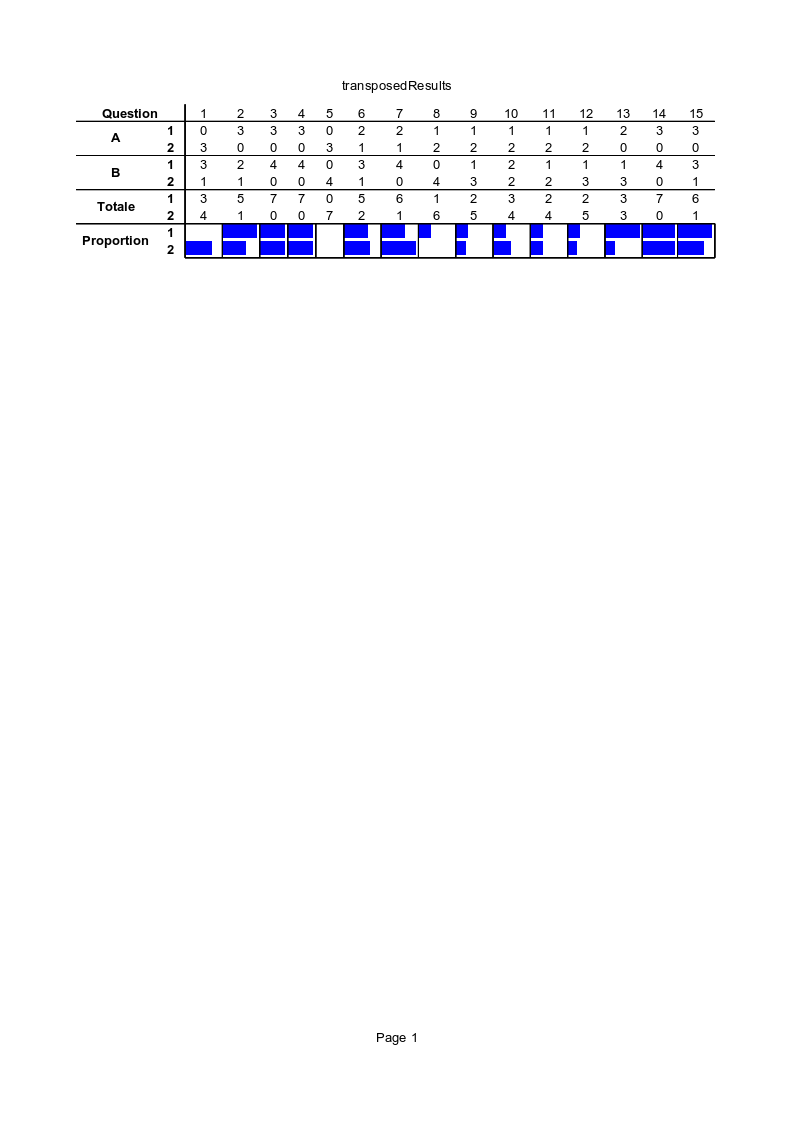
\includegraphics[scale=0.5]{transposedResults}%\hspace*{4cm}
\end{center}
  \end{frame}


%% Analyse
\section{Analyse}
\begin{frame}
  \frametitle{Analyse}
  \begin{itemize}
  \item   ss
  \end{itemize}
\end{frame}

%% Conclusions
\section{Conclusions}
\subsection{Conclusions d'étude pilote}
\begin{frame}
\frametitle{Conclusions d'étude pilote}
  \begin{itemize}
  \item Les résultats nous donne confiance que cette approche pourrait fonctionner.
  \item Nous voyons que certains questions ne sont pas bonnes - tout le monde
    choisit la même réponse. Ces questions devraient être changées pour la suite.
  \end{itemize}
\end{frame}

\subsection{La suite}
\begin{frame}
  \frametitle{La suite}
  \begin{itemize}
  \item   
  \end{itemize}
\end{frame}


\section{Annexes}
%% Bibliographie
\begin{frame}
\frametitle{Bibliographie}
\end{frame}

\end{document}
